\documentclass[12pt]{article}
\usepackage{makecell}
\usepackage{hyphenat}
\usepackage[utf8]{vietnam}
\usepackage[vietnamese=nohyphenation]{hyphsubst}
\usepackage[vietnamese]{babel}
\usepackage[table,dvipsnames]{xcolor} % Required for row coloring
\usepackage{booktabs} % Required for nicer horizontal lines
\usepackage{ragged2e}
\usepackage{caption}
\usepackage{subcaption}
\usepackage{float}
\usepackage{amsmath,amssymb,amsfonts}
\usepackage{graphicx}
\usepackage{adjustbox}
\usepackage{multicol}
\usepackage[inline,shortlabels]{enumitem}
\usepackage{setspace}
\usepackage{longtable}
\usepackage{bm} 
\usepackage[inkscapelatex=false]{svg}
\usepackage{titling}
\usepackage{tabularx}
\usepackage[T1]{fontenc}
\usepackage{lmodern,mathrsfs}
% \usepackage[draft]{hyperref}
\usepackage{hyperref}
\usepackage{xparse}
\usepackage{fontawesome5}
\usepackage[most]{tcolorbox}
\usepackage{tikz}
\usepackage[framemethod=TikZ]{mdframed}
\usetikzlibrary{matrix, fit, shadows, positioning, arrows.meta, calc, shapes.geometric, backgrounds, shapes.symbols}
\usepackage{paracol}
\usepackage{bbm}
\usepackage{pgfplots}
\usepackage{siunitx}
\usepackage{multirow}
\usepackage[dvipsnames]{xcolor}



%  biblatex (thay cho IEEEtran.bst) ------------------------------------
\usepackage[
    backend=bibtex,
    style=ieee,
    citestyle=numeric-comp,
    maxnames=1,     % chỉ hiển thị 1 tên tác giả, phần còn lại thành ``et al."
    minnames=1,
    uniquelist=false,
    hyperref=false
]{biblatex}
\usepackage{forest}
\addbibresource{references.bib}
\DefineBibliographyStrings{english}{
  andothers = {et\addabbrvspace al\adddot}
}
% Danh mục tham khảo có tên tiếng Việt nên KHÔNG chuyển sang tiếng Anh ở đây
% (bản mẫu có dòng \AtBeginBibliography{\selectlanguage{english}}, làm lỗi chữ Việt trong danh mục)

% -----------------------------------------------------------------
\AtBeginDocument{\renewcommand\refname{}}

\usepackage[toc,page]{appendix}
\renewcommand{\appendixtocname}{Phụ lục}      
\renewcommand{\appendixpagename}{Phụ lục}

\usepackage{xurl}
\setlength{\headheight}{14.5pt}
\setlength{\topmargin}{-.5in} \setlength{\textheight}{9.25in}
\setlength{\oddsidemargin}{-0.1in} \setlength{\textwidth}{6.8in}

\usepackage{tocloft}
\renewcommand{\cfttoctitlefont}{\Huge\bfseries}
\setlength{\cftaftertoctitleskip}{2em}
\setlength{\cftbeforesubsecskip}{7pt} % giãn cách subitem mục lục
\renewcommand{\cftsecleader}{\cftdotfill{\cftdotsep}}
\setlength{\cftsecnumwidth}{3em}
\renewcommand{\cftsecaftersnum}{\quad}
\renewcommand{\cftsubsecleader}{\cftdotfill{\cftdotsep}}
\setlength{\cftsubsecnumwidth}{4em}
\renewcommand{\cftsubsecaftersnum}{\quad}
\renewcommand{\cftsubsubsecleader}{\cftdotfill{\cftdotsep}}
\setlength   {\cftsubsubsecnumwidth}{5em}  
\renewcommand{\cftsubsubsecaftersnum}{\quad}

\PassOptionsToPackage{vietnamese.licr}{babel}
\usepackage{vipythonhighlight}
\usepackage{tvietlistings}
\newcounter{mycounter}
\newcommand\showmycounter{\stepcounter{mycounter}\themycounter}
\usepackage{lipsum}
\newcommand\showlips{\stepcounter{mycounter}\lipsum[\value{mycounter}]}

%--------------------------------------------------------------------
\usepackage{framed}
\usepackage{fancyhdr}
\usepackage{upquote}
\usepackage{listings}	 
	    

\usepackage[toc, nonumberlist, style=super]{glossaries}
\makenoidxglossaries

\newglossarystyle{clean3col}{%
    % 1) Table layout: 3 columns
    \renewenvironment{theglossary}%
    {%
      \begin{longtable}{@{}
        >{\setlength{\parindent}{0pt}\RaggedRight\arraybackslash}p{0.2\linewidth}
        >{\setlength{\parindent}{0pt}\RaggedRight\arraybackslash}p{0.23\linewidth}
        >{\setlength{\parindent}{0pt}\RaggedRight\arraybackslash}p{0.52\linewidth}
      @{}}%
    }%
    {\end{longtable}}%

    % 2) Header row
    \renewcommand{\glossaryheader}{%
        \bfseries Thuật ngữ &
        \bfseries Tạm dịch &
        \bfseries Mô tả \\
        \midrule
        \endhead
    }%

    % 3) Each entry row
    \renewcommand{\glossentry}[2]{%
        \itshape \glstarget{##1}{\glossentryname{##1}} &
        \glsentryuseri{##1} &
        \glossentrydesc{##1} \\
        \addlinespace[6pt]
    }%
}


% Color --------------------------------------------------------------------
\usepackage{epigraph}
\usepackage{titlesec}

\definecolor{codebackground}{RGB}{250, 250, 250}
\definecolor{codecomment}{RGB}{34, 139, 34}
\definecolor{codekeyword}{RGB}{0, 0, 255}
\definecolor{codestring}{RGB}{255, 0, 0}
\definecolor{codeidentifier}{RGB}{0, 0, 0}
\definecolor{codelinenumbers}{RGB}{90, 90, 90}

\definecolor{codegreen}{rgb}{0,0.6,0}
\definecolor{codegray}{rgb}{0.5,0.5,0.5}
\definecolor{codepurple}{rgb}{0.58,0,0.82}
\definecolor{backcolour}{rgb}{0.95,0.95,0.92}

\definecolor{aivnGreen}{RGB}{52,79,30}  
\definecolor{aivnCodeOutputColor}{RGB}{11,83,148}  
\definecolor{captiongray}{gray}{0.15} 
\definecolor{captionbg}{RGB}{250,250,250}

\definecolor{foldercolor}{RGB}{0, 102, 204}
\definecolor{filecolor}{RGB}{104, 104, 104}
\definecolor{scriptcolor}{RGB}{180, 50, 50}
\definecolor{pythoncolor}{RGB}{0, 128, 128}

% --- Extra Brand colors for the table ---
\definecolor{brandIndigo}{HTML}{333D91} 
\definecolor{rowLavender}{HTML}{EEECFA}
\setlength{\parskip}{0.3em}

% Table
\newtcolorbox{captionbelowboxaivn}{
    colback=aivnGreen,
    colframe=aivnGreen,
    boxrule=0pt,
    arc=4pt,
    left=4pt,
    right=4pt,
    top=2pt,
    bottom=2pt,
    width=\linewidth,
    boxsep=4pt,
    halign=center,
    % fontupper=\bfseries\color{white}
    fontupper=\color{white}
}

% Figure
\newtcolorbox{figurecardcaptionaivn}{
  colback=aivnGreen,        % Màu nền (background color)
  colframe=aivnGreen,       % Màu viền box (border color)
  boxrule=0pt,              % Độ dày viền box (0pt = không viền)
  arc=2pt,                  % Độ bo góc (2pt là bo nhẹ, tăng để bo tròn hơn)
  top=3pt,                  % Padding phía trên nội dung
  bottom=3pt,               % Padding phía dưới nội dung
  left=10pt,                % Padding bên trái
  right=10pt,               % Padding bên phải
  width=\linewidth,         % Chiều rộng bằng toàn bộ dòng
  fontupper=\small\fontsize{11pt}{13pt}\selectfont\color{white} 
}

% Tạo counter riêng
\newcounter{hinh}
% Định nghĩa macro caption Hình
\newcommand{\capfig}[1]{%
  \refstepcounter{hinh}%
  % \textbf{Hình~\thehinh:}~#1
    Hình~\thehinh:~#1
}

\newtcolorbox{figurecaptionmodern1}{
  colback=captionbg,
  colframe=aivnGreen,
  boxrule=0.3pt,
  bottomrule=0.3pt,  
  toptitle=0pt,
  bottomtitle=0pt,
  left=6pt,
  right=6pt,
  top=4pt,
  bottom=2pt,
  width=\linewidth,
  fontupper=\small\fontsize{11pt}{13pt}\selectfont\color{black},
  halign=center
}

\newtcolorbox{figurecaptionmodern}{
  colback=captionbg,
  colframe=aivnGreen,
  boxrule=0.3pt,
  bottomrule=0.3pt,  
  toptitle=0pt,
  bottomtitle=0pt,
  left=6pt,
  right=6pt,
  top=4pt,
  bottom=2pt,
  width=\linewidth,
  fontupper=\small\fontsize{11pt}{13pt}\selectfont\color{black},
  halign=justify
}

% Code Block -----------------------------------------------------------------
\newtcolorbox{aivncodebox}[1][]{%
  enhanced,
  colback=gray!10,
  colframe=aivnGreen,
  coltitle=white,
  colbacktitle=aivnGreen,
  title=#1,
  fonttitle=\bfseries\sffamily,
  listing only,
  breakable,
  listing engine=listings,
  listing options={
    language=Python,
    basicstyle=\ttfamily\footnotesize,
    commentstyle=\color{ForestGreen},
    keywordstyle=\color{blue},
    stringstyle=\color{red!70!black},
    numbers=left, upquote=true,
    numberstyle=\tiny\color{gray},
    numbersep=5pt,
    breaklines=true,
    showstringspaces=false,
    xleftmargin=1.5em,
    framexleftmargin=1.5em
  }
}

% Code Output Block -----------------------------------------------------------------
\newtcolorbox{aivnCodeOutput}[1][]{%
  enhanced,
  colback=gray!10,
  colframe=aivnCodeOutputColor,
  coltitle=white,
  colbacktitle=aivnCodeOutputColor,
  title=#1,
  fonttitle=\bfseries\sffamily,
  listing only,
  breakable,
  listing engine=listings,
  listing options={
    language=Python,
    basicstyle=\ttfamily\footnotesize,
    commentstyle=\color{ForestGreen},
    keywordstyle=\color{blue},
    stringstyle=\color{red!70!black},
    numbers=left,
    numberstyle=\tiny\color{gray},
    numbersep=5pt,
    breaklines=true,
    showstringspaces=false,
    xleftmargin=1.5em,
    framexleftmargin=1.5em
  }
}

% Last argument allows more tcolorbox options to be added

% --- Guideline/Tip box ---
\newtcolorbox{guidelinebox}[2][]{
    enhanced, colback=yellow!10!white, colframe=orange!90!black, boxrule=1pt, arc=4pt,
    fonttitle=\bfseries, attach boxed title to top left={yshift=-2mm, xshift=3mm},
    colbacktitle=orange!90!black, coltitle=white,
    title=\faLightbulb\hspace{1mm} #2, #1
}

\newtcolorbox{notebox}[1][]{
  enhanced,  colback=yellow!10, colframe=orange!80, boxrule=1pt, 
  arc=4pt, fontupper=\small, attach boxed title to top left={yshift=-2mm, xshift=3mm},
  colbacktitle=orange!80,  coltitle=white, fonttitle=\bfseries,  
  title=\faInfoCircle~\textbf{Lưu ý},  #1
}

\newtcolorbox{infobox}[1]{%
    enhanced, 
    breakable, 
    colback=green!3, 
    colframe=green!3, 
    arc=5pt,
    borderline west={3pt}{0pt}{aivnGreen},
    attach boxed title to top left={ 
        yshift*=-\tcboxedtitleheight/2, 
        xshift=-0.1em 
    },
    colbacktitle=aivnGreen, %
    coltitle=white, 
    fonttitle=\bfseries, 
    boxed title style={ 
        arc=4pt, 
        top=2pt, 
        bottom=2pt,
        left=8pt,
        right=8pt,
    },
    title={\faInfoCircle\quad #1}
}
\newtcolorbox{examplebox}[1]{%
    enhanced,
    breakable,
    colback=brandIndigo!5,      
    colframe=brandIndigo!5,     
    arc=5pt,
    borderline west={3pt}{0pt}{brandIndigo}, 
    attach boxed title to top left={
        yshift*=-\tcboxedtitleheight/2,
        xshift=-0.1em
    },
    colbacktitle=brandIndigo,   
    coltitle=white,
    fonttitle=\bfseries,
    boxed title style={
        arc=4pt,
        top=2pt,
        bottom=2pt,
        left=8pt,
        right=8pt,
    },
    title={\faLightbulb\quad #1} 
}
% Misconception / warning box (dùng trong mục Hiểu về bối cảnh sản xuất thép) --
\newtcolorbox{misconceptionbox}[1]{%
    enhanced,
    breakable,
    colback=red!4,
    colframe=red!55!black,
    boxrule=1pt,
    arc=4pt,
    fontupper=\small,
    left=8pt, right=8pt, top=4pt, bottom=4pt,
    title={\faExclamationTriangle\quad #1},
    fonttitle=\bfseries,
    coltitle=red!45!black,
    colbacktitle=red!4,
    boxed title style={boxrule=0pt, arc=0pt, left=0pt, right=0pt, top=0pt, bottom=0pt},
    attach boxed title to top left={yshift=-2mm, xshift=3mm}
}
% Prompt Block ---------------------------------------------------------------
\definecolor{promptBlue}{HTML}{2F5D8C}
\definecolor{promptBg}{HTML}{F6F9FC}
\definecolor{promptBorder}{HTML}{B7C9DC}

% Dùng cho prompt đã viết theo cú pháp LaTeX bình thường
\newtcolorbox{promptbox}[1][Prompt]{%
    enhanced,
    breakable,
    colback=promptBg,
    colframe=promptBorder,
    coltitle=white,
    colbacktitle=promptBlue,
    fonttitle=\bfseries\sffamily,
    title={#1},
    boxrule=0.8pt,
    arc=4pt,
    left=8pt,
    right=8pt,
    top=2pt,
    bottom=1pt,
    before skip=8pt,
    after skip=8pt,
    borderline west={3pt}{0pt}{promptBlue},
    fontupper=\small\sffamily,
}

% Dùng cho prompt raw: giữ nguyên xuống dòng, không highlight keyword
\newtcblisting{promptboxraw}[1][Prompt]{%
    enhanced,
    breakable,
    listing only,
    listing engine=listings,
    colback=promptBg,
    colframe=promptBorder,
    coltitle=white,
    colbacktitle=promptBlue,
    fonttitle=\bfseries\sffamily,
    title={#1},
    boxrule=0.8pt,
    arc=4pt,
    left=8pt,
    right=8pt,
    top=-4pt,
    bottom=-4pt,
    before skip=4pt,
    after skip=4pt,
    borderline west={3pt}{0pt}{promptBlue},
    listing options={
        language={},
        basicstyle=\small\ttfamily,
        columns=fullflexible,
        keepspaces=true,
        breaklines=true,
        showstringspaces=false,
        numbers=none,
        frame=none,
        keywordstyle=\color{black},
        commentstyle=\color{black},
        stringstyle=\color{black},
        identifierstyle=\color{black}
    }
}


%--------------------------------------------------------------------
\lstdefinestyle{mystyle}{
    backgroundcolor=\color{codebackground},
    commentstyle=\color{codecomment},
    keywordstyle=\color{codekeyword},
    stringstyle=\color{codestring},
    identifierstyle=\color{codeidentifier},
    basicstyle=\ttfamily\footnotesize,
    breakatwhitespace=false,
    breaklines=true,
    captionpos=b,
    keepspaces=true,
    numbers=left,
    numberstyle=\tiny\color{codelinenumbers}, 
    numbersep=5pt,
    showspaces=false,
    showstringspaces=false,
    showtabs=false,
    tabsize=2
}

\lstset{style=mystyle}

\hypersetup{
    colorlinks=true,
    linkcolor=black,
    filecolor=magenta,    
    citecolor=green,
    urlcolor=blue,
    pdftitle={Đối soát doanh thu Nexa Home 2025: báo cáo nhanh và sổ cái},
    pdfpagemode=FullScreen,
}

%--------------------------------------------------------------------
\newcounter{choice}
\renewcommand\thechoice{($\alph{choice}$)}
\newcommand\choicelabel{\thechoice}

%--------------------------------------------------------------------
\newenvironment{choices}%
  {\list{\choicelabel}%
     {\usecounter{choice}\def\makelabel##1{\hss\llap{##1}}%
       \settowidth{\leftmargin}{W.\hskip\labelsep\hskip 0 em}%
       \def\choice{%
         \item
       } % choice
       \labelwidth\leftmargin\advance\labelwidth-\labelsep
       \topsep=0pt
       \partopsep=0pt
     }%
  }%
  {\endlist}
  
%--------------------------------------------------------------------
\def\CChoice{%
      \choice
      \addanswer{\theenumi}{\thechoice}%
    }
    \let\CChoice\CChoice
%    \par % Uncomment this to have choices always start a new line
   % \let\par\@empty
    % If we're continuing the textbf containing the question,
    % then leave a bit of space before the first choice:
    \ifvmode\else\enskip\fi
    \ignorespaces
  %
  {}
\makeatother
\newbox\allanswers
\setbox\allanswers=\hbox{}
\newcommand{\addanswer}[2]{%
  \global\setbox\allanswers=\hbox{\unhbox\allanswers \quad #1.~#2}%
}
\newcommand{\showanswers}{%
  \vfill
  \begin{center}
    Answers
  \end{center}
  \unhbox\allanswers
}

\makeatletter
\newenvironment{multichoices}[1][1]{%
\begin{multicols}{#1}}{%
\end{multicols}}
\makeatother

\pagestyle{fancy}

\DeclareMathOperator*{\argmax}{arg\,max}
\DeclareMathOperator*{\argmin}{arg\,min}
\DeclareMathOperator{\E}{\mathbb{E}}

% Outline --------------------------------------------------------------------
% Section numbering ----------------------------------------------------------
\renewcommand{\thesection}{\Roman{section}.}
\renewcommand{\thesubsection}{\thesection\arabic{subsection}.}
\renewcommand{\thesubsubsection}{\thesubsection\arabic{subsubsection}.}

% Phân chia lớn: Mục A (nền tảng lý thuyết) / Mục B (thực hành) --------------
% \part{} không ảnh hưởng tới việc đánh số La Mã liên tục của \section.
\renewcommand{\thepart}{\Alph{part}}
\titleformat{\part}[display]
  {\centering\normalfont\color{aivnGreen}}
  {\bfseries\Large MỤC \thepart}
  {0.4em}
  {\bfseries\huge}
  [\vspace{0.4em}{\color{aivnGreen}\titlerule[1.2pt]}\vspace{1.8em}]

% Paper-like section title sizes --------------------------------------------
% Title paper: 17pt
% Section should be clearly smaller than title but still prominent.
\titleformat{\section}
  {\normalfont\fontsize{16pt}{20pt}\selectfont\bfseries}
  {\thesection}
  {0.85em}
  {}

\titleformat{\subsection}
  {\normalfont\fontsize{14pt}{16pt}\selectfont\bfseries}
  {\thesubsection}
  {0.75em}
  {}

\titleformat{\subsubsection}
  {\normalfont\fontsize{12pt}{15pt}\selectfont\bfseries}
  {\thesubsubsection}
  {0.65em}
  {}

% Paper-like compact spacing -------------------------------------------------
\titlespacing*{\section}
  {0pt}
  {1.25em plus 0.2em minus 0.1em}
  {0.65em plus 0.1em minus 0.1em}

\titlespacing*{\subsection}
  {0pt}
  {1.0em plus 0.2em minus 0.1em}
  {0.45em plus 0.1em minus 0.1em}

\titlespacing*{\subsubsection}
  {0pt}
  {0.85em plus 0.15em minus 0.1em}
  {0.35em plus 0.1em minus 0.1em}


% Logo + Title ---------------------------------------------------------------

\setlength{\droptitle}{-7em}

% Title horizontal rule
\newcommand{\TitleRule}{%
  \rule{0.90\textwidth}{0.6pt}
}

% Chiều cao vùng title giữa 2 rule
\newlength{\TitleBlockHeight}
\setlength{\TitleBlockHeight}{2.2cm}

\pretitle{%
  

  % Logo row
  \begin{tabular}{@{}c@{\hspace{1.0em}}c@{\hspace{1.0em}}c@{}}
    \raisebox{-0.35\height}{
\includegraphics[height=2.0cm]{Figures/eda_logo.png}}    
  \end{tabular}

  %\vspace{0.2em}

\begin{center}
  \TitleRule
  \par\nointerlineskip
}

\title{%
  \parbox[c][\TitleBlockHeight][c]{0.90\textwidth}{%
    \centering
    {\fontsize{20pt}{24pt}\selectfont\bfseries Đối soát doanh thu Nexa Home năm 2025:\\ vì sao sổ cái thấp hơn báo cáo nhanh 2,43 triệu USD}\\[.5ex]
  }%
}

\posttitle{%
  \par\nointerlineskip
  \TitleRule
  \end{center}
}

\preauthor{%
  \begin{center}
  \fontsize{11pt}{13pt}\selectfont
}

\author{%
  \textbf{Lê Nguyễn Phước Thành}
  \hspace{3em}
  \textbf{(Thành viên 2)}
  \hspace{3em}
  \textbf{(Thành viên 3)}
}

\postauthor{%
  \par\vspace{0.6em}
  {\fontsize{11pt}{13pt}\selectfont \textbf{ Mentor:} \textbf{(tên mentor)}}
  \par
  \end{center}
}

\date{}
% Header --------------------------------------------------------------------
\pagestyle{fancy}
\fancyhf{}
\lhead{\href{https://www.facebook.com/aivietnam.edu.vn}{\textcolor{aivnGreen}{\bfseries End-to-End Data Analytics}}}
\rhead{\href{https://eda.aivietnam.edu.vn/}{\textcolor{aivnGreen}{\bfseries eda.aivietnam.edu.vn}}}
\fancyfoot[r]{\textcolor{aivnGreen}{\bfseries Trang \thepage}}
\fancyfoot[l]{%
  \href{https://zalo.me/84911118758}{%
    \textcolor{aivnGreen}{\bfseries SĐT/Zalo: 0911118758 (Dr. Hồng Phúc)}%
  }%
}
\renewcommand{\headrulewidth}{1.0pt}
\renewcommand{\headrule}{{\color{aivnGreen}\hrule width\headwidth height\headrulewidth \vskip-\headrulewidth}}

\renewcommand{\footrulewidth}{1.0pt}
\renewcommand{\footrule}{{\color{aivnGreen}\hrule width\headwidth height\headrulewidth \vskip-\headrulewidth}}


\fancypagestyle{firstpage}{
    \fancyhf{}
    \fancyfoot[r]{\textcolor{aivnGreen}{\bfseries Trang \thepage}}
    \fancyfoot[l]{%
      \href{https://zalo.me/84911118758}{%
        \textcolor{aivnGreen}{\bfseries SĐT/Zalo: 0911118758 (Dr. Hồng Phúc)}%
      }%
    }
    \renewcommand{\headrulewidth}{0pt}
    \renewcommand{\footrulewidth}{1.0pt}
    \renewcommand{\footrule}{%
        {\color{aivnGreen}\hrule width\headwidth height\footrulewidth}
    }
}

% Cho phép gõ dấu trừ Unicode (U+2212) trong lời văn ----------------------------
\DeclareUnicodeCharacter{2212}{\ensuremath{-}}
% Bảng: chú thích "Bảng N:" giống \capfig của hình ------------------------------
\newcounter{bang}
\newcommand{\captab}[1]{\refstepcounter{bang}\par\noindent\textbf{Bảng~\thebang:}~#1\par\smallskip}
% Nhãn nguồn số liệu (xem docs/quy_uoc_va_so_chuan.md) -------------------------
\newcommand{\nguon}[1]{\textsf{\small[#1]}}
% Ghi chú phần chưa viết (phải hết ở bản nộp) -------------------------------------
\newcommand{\choviet}[1]{\begin{notebox}Phần này viết ở plan \texttt{#1}.\end{notebox}}
% Số liệu sinh tự động từ file Excel Power Query ---------------------------------
\newcommand{\SoFlashNam}{31.124.401}
\newcommand{\SoSoCaiNam}{28.698.496,23}
\newcommand{\SoChenhLechNam}{$-$2.425.904,77}
\newcommand{\SoPctNam}{$-$7,79\%}
\newcommand{\SoThangThap}{11}
\newcommand{\SoThangBaChenhLech}{99.017,53}
\newcommand{\SoThangBaPct}{4,95\%}
\newcommand{\SoThangLechNhatPct}{tháng 4 ($-$13,31\%)}
\newcommand{\SoThangLechNhatTien}{tháng 2 ($-$387.252,01)}
\newcommand{\SoOnlineChenhLech}{$-$1.548.553,02}
\newcommand{\SoOnlineTyTrong}{64\%}
\newcommand{\SoChuaGanKenh}{1.250,00}
\newcommand{\SoQCDat}{13}
\newcommand{\SoQCTong}{13}
\newcommand{\SoDongGiaoDich}{26.565}
\newcommand{\SoDongPOS}{17.124}
\newcommand{\SoDongWEB}{9.441}
\newcommand{\SoKiemTraChatLuong}{13}
\newcommand{\SoKiemTraCanXem}{4}
\newcommand{\SoOCuaHang}{5.120}
\newcommand{\SoOCuaHangKhop}{5.118}
\newcommand{\SoOCuaHangLech}{2}
\newcommand{\SoOLechNgayBanNam}{2.929}
\newcommand{\SoOThangMuoiMot}{453}
\newcommand{\SoOLechNgayBanTMM}{347}
\newcommand{\SoCHVuotTruocTMM}{21}
\newcommand{\SoCHVuotSauTMM}{1}
\newcommand{\SoNXNamBayLech}{$-$7.227,56}
\newcommand{\SoNXNamBayPct}{$-$74,5\%}
\newcommand{\SoNXNamBaySoCai}{9.694,98}
\newcommand{\SoNXNamBayPOS}{16.922,54}
\newcommand{\SoNXNamBayTruoc}{$-$12.446,87}
\newcommand{\SoNXKhongTamTruoc}{$-$716,19}
\newcommand{\SoNXKhongTamSau}{$-$0,01}
\newcommand{\SoCHVuotTruocNam}{137}
\newcommand{\SoCHVuotSauNam}{2}
\newcommand{\SoCapThang}{tháng 5 sang tháng 6: 41.464,78 USD (65 dòng); tháng 8 sang tháng 9: 75.240,30 USD (101 dòng); tháng 11 sang tháng 12: 80.588,85 USD (101 dòng)}
\newcommand{\SoSoCapThang}{3}
\newcommand{\SoDongSangThang}{267}


\begin{document}
\maketitle
\thispagestyle{firstpage}
\vspace{-3em}

% Tóm tắt cho Giám đốc Tài chính: đọc trong 1 phút biết lệch bao nhiêu, vì sao, ai cần làm gì
\begin{infobox}{Tóm tắt}
Năm 2025, báo cáo nhanh doanh số của phòng Kinh doanh (Flash) ghi \SoFlashNam{} USD (đô la Mỹ), sổ cái của phòng Tài chính ghi \SoSoCaiNam{} USD. Chênh lệch sổ cái $-$ Flash là \SoChenhLechNam{} USD, tức \SoPctNam{} so với Flash \nguon{QC}. Sổ cái thấp hơn Flash ở \SoThangThap{}/12 tháng; riêng tháng 3 sổ cái cao hơn \SoThangBaChenhLech{} USD \nguon{BR-Tổng}. Kênh online chiếm \SoOnlineTyTrong{} phần chênh lệch \nguon{BR-WEB}.

\smallskip
\noindent\textit{Phần trả lời ``vì sao lệch, khoản nào là lỗi, ai cần sửa gì'' được viết sau khi xong bảng cầu nối (plan \texttt{conclusions}).}
\end{infobox}


\tableofcontents
\newpage

\section{Vấn đề và câu hỏi phân tích}

\subsection{Hai con số cho cùng một năm}

Nexa Home bán đồ gia dụng và điện tử qua 57 cửa hàng ở 8 nước và một website. Đầu tháng 1/2026, hai phòng gửi lên Giám đốc Tài chính hai con số doanh thu năm 2025 khác nhau:
\begin{itemize}
  \item \textbf{Flash} (báo cáo nhanh doanh số của phòng Kinh doanh): \SoFlashNam{} USD.
  \item \textbf{Sổ cái} (GL -- General Ledger, sổ kế toán của phòng Tài chính): \SoSoCaiNam{} USD.
\end{itemize}
Chênh lệch là \SoChenhLechNam{} USD, tức \SoPctNam{} so với Flash \nguon{QC}.

Đây là một bài \textbf{đối soát}: so hai nguồn số để tìm ra chỗ lệch, đo từng khoản lệch, tách khoản nào là quy tắc ghi nhận hợp lệ với khoản nào là lỗi, và đề xuất thay đổi quy trình. Bài này \textbf{không} phân tích tăng trưởng, sản phẩm bán chạy hay mùa vụ.

\subsection{Ba câu hỏi của Giám đốc Tài chính}

\begin{enumerate}
  \item Flash và sổ cái lệch bao nhiêu, theo tháng và theo kênh bán?
  \item Chênh lệch gồm những khoản nào, mỗi khoản bao nhiêu tiền, khoản nào là lỗi?
  \item Quy trình cần đổi gì để tháng sau đối soát nhanh hơn?
\end{enumerate}

\subsection{Ba câu hỏi riêng của nhóm}

Ba câu hỏi của Giám đốc Tài chính trả lời "lệch bao nhiêu, gồm gì". Nhóm đặt thêm ba câu hỏi để biết \textbf{phần nào cần hành động}, mỗi câu đo được bằng một con số trong bảng của nhóm.

\captab{Câu hỏi riêng của nhóm, thước đo và nơi lấy số}\nopagebreak[4]
\begin{longtable}{@{}p{0.5cm} p{6.2cm} p{4.6cm} p{3.6cm}@{}}
\toprule
\# & Câu hỏi & Đo bằng & Lấy số ở \\
\midrule
\endhead
Q1 & Trong \SoChenhLechNam{} USD chênh lệch, bao nhiêu là hợp lệ do hai bên ghi nhận khác nhau, bao nhiêu là lỗi dữ liệu cần sửa, bao nhiêu chưa giải thích được? & Tổng các khoản của bảng cầu nối theo 4 nhóm, và tỷ lệ trên độ lớn chênh lệch & Bảng cầu nối toàn công ty \nguon{BR-Tổng} \\
\midrule
Q2 & Sau khi trừ các khoản do quy tắc ghi nhận, tháng nào vẫn còn lệch vượt ngưỡng 200 USD, tức là tháng nào thật sự cần điều tra? & "Chênh lệch còn lại" từng tháng = chênh lệch $-$ các khoản quy tắc ghi nhận & Bảng cầu nối 12 tháng \nguon{BR-Tổng} \\
\midrule
Q3 & Các khoản lệch do thời điểm ghi nhận có tự bù trừ ở tháng sau không, và bao nhiêu tiền vắt qua năm nên không tự bù trong năm 2025? & Cặp tháng âm/dương của khoản lệch ngày ghi sổ và lệch thời điểm online; phần đơn đặt năm này giao năm sau & Bảng đối soát cửa hàng, online \nguon{RC-CH}, \nguon{RC-WEB} \\
\bottomrule
\end{longtable}

\subsection{Quy ước chốt trước khi tính}

Các quy ước dưới đây được chốt và lưu lên GitHub ngày 15/10/2026, \textbf{trước khi tính bất kỳ con số nào}, theo nguyên tắc "đặt ngưỡng trước khi nhìn số" của đề \cite{slide_project1}.

\captab{Quy ước tính}\nopagebreak[4]
\begin{longtable}{@{}p{4.2cm} p{10.8cm}@{}}
\toprule
Nội dung & Thống nhất \\
\midrule
\endhead
Nguồn chuẩn & Sổ cái: đã khóa sổ từng tháng, ghi theo chuẩn mực kế toán VAS 14 \cite{vas14}, có giấy tờ làm căn cứ. \\
Chênh lệch & Chênh lệch = Sổ cái $-$ Flash. Trong bảng cầu nối, khoản nào làm Flash cao hơn sổ cái thì ghi số âm. \\
\% chênh lệch & Trên thẻ số liệu chính: chia cho Flash. Khi đánh dấu cửa hàng $\times$ tháng vượt ngưỡng: chia cho |sổ cái|. \\
Ngưỡng phải giải thích & |Chênh lệch| $> 200$ USD \textbf{và} |\% chênh lệch| $> 1\%$, tính cho một cửa hàng trong một tháng, sau khi đã đưa hai bên về cùng cách tính. \\
Sai số chấp nhận & Làm tròn $\le 5$ USD mỗi tháng; dòng kiểm tra của bảng cầu nối $\le 1$ USD. \\
Thứ tự các bước cầu nối & Flash $\rightarrow$ chiết khấu $\rightarrow$ dòng POS trùng $\rightarrow$ đơn hủy $\rightarrow$ lệch thời điểm online $\rightarrow$ lệch ngày ghi sổ cửa hàng $\rightarrow$ lỗi chuyển dữ liệu $\rightarrow$ hàng trả $\rightarrow$ phí vận chuyển $\rightarrow$ (chuyển kênh, chỉ ở bảng theo kênh) $\rightarrow$ tỷ giá $\rightarrow$ làm tròn $\rightarrow$ chưa giải thích $\rightarrow$ sổ cái. Trừ chiết khấu trước để dòng trùng và đơn hủy được tính theo giá sau giảm giá, giống cách sổ cái ghi. \\
Bút toán ADJ-0925 & Bút toán điều chỉnh 1.250 USD không có giấy tờ: luôn để ở dòng "Chưa giải thích được", không gộp vào khoản khác. \\
\bottomrule
\end{longtable}

\begin{notebox}
Ngày 18/10/2026 nhóm sửa một quy ước: dòng tỷ giá tính từ nội tệ chia tỷ giá, chưa làm tròn; phần sổ cái làm tròn từng bút toán đưa vào dòng làm tròn. Cách này đúng định nghĩa của đề (slide 34) và cho dòng làm tròn cả năm +1,01 USD như slide 32. Lý do và so sánh ở Phụ lục~D.
\end{notebox}

\section{Dữ liệu và chuẩn bị}

\subsection{Bốn nguồn dữ liệu}

Bốn nguồn ghi doanh thu ở bốn mức chi tiết khác nhau, nên không thể ghép từng dòng của nguồn này với từng dòng của nguồn kia (Bảng~\ref{tab:nguon}). Dữ liệu là bộ giả lập dựng từ Contoso Data Generator V2 \cite{contoso_v2}.

\captab{Bốn nguồn dữ liệu: một dòng là gì, khóa, ngày, tiền, dấu}\label{tab:nguon}\nopagebreak[4]
{\small
\begin{longtable}{@{}L{2.6cm} L{3.4cm} L{2.4cm} L{3.0cm} L{3.4cm}@{}}
\toprule
Nguồn & Một dòng là & Khóa & Ngày & Tiền, dấu \\
\midrule
\endhead
POS (Point of Sale, bán tại cửa hàng) & 1 món hàng trên 1 hóa đơn & \texttt{receipt\_no} + \texttt{line\_no} & Ngày bán & Nội tệ của nước có cửa hàng; dương \\
\midrule
WEB (đơn online) & 1 đơn hàng & \texttt{web\_order\_id} & Ngày đặt, ngày giao, ngày trả (kiểu Mỹ MM/DD/YYYY) & Tiền khách trả; dương \\
\midrule
Sổ cái & 1 bút toán, gộp cửa hàng $\times$ ngày ghi sổ hoặc ngày giao $\times$ loại tiền & \texttt{journal\_id} & Ngày ghi sổ & Nội tệ và USD theo tỷ giá cuối tháng; doanh thu âm, hàng trả dương \\
\midrule
Flash & 1 tháng $\times$ 1 kênh $\times$ 1 thị trường & Không có & Tháng đặt hàng & USD theo tỷ giá ngày đặt, làm tròn đến USD; dương \\
\bottomrule
\end{longtable}}

\textbf{Ai giữ nguồn nào.} File POS và file đơn online được xuất từ hệ thống bán hàng tại cửa hàng và hệ thống quản lý đơn online (OMS -- Order Management System); bộ phận vận hành bán hàng chịu trách nhiệm trạng thái đơn, ngày giao, hàng trả và việc xuất file. Sổ cái do phòng Tài chính giữ, gồm cả bút toán tay, bút toán bổ sung và quy đổi tỷ giá. Flash do phòng Kinh doanh lập ngày 05/01/2026; file đơn online được trích xuất ngày 15/01/2026. Khi một con số lệch, bảng này cho biết cần hỏi bộ phận nào.

\subsection{Mỗi bên ghi doanh thu thế nào: năm lý do lệch}

Hai bên đều đúng theo cách của mình nhưng khác nhau ở năm điểm (đề gọi là ``năm trục khác biệt''). Mục~IV chứng minh từng lý do bằng số trên dữ liệu.

\captab{Quy tắc ghi nhận của từng bên}\nopagebreak[4]
{\small
\begin{longtable}{@{}L{2.6cm} L{4.0cm} L{4.2cm} L{4.0cm}@{}}
\toprule
Lý do lệch & Flash & Sổ cái -- cửa hàng & Sổ cái -- online \\
\midrule
\endhead
Thời điểm & Ngày khách đặt hàng & Ngày ghi sổ; bán ngày nghỉ thì ghi ngày làm việc kế tiếp & Ngày giao thành công; hàng trả ghi giảm vào ngày nhận hàng trả \\
Giá trị & Giá niêm yết, trước giảm giá & Sau giảm giá & Sau giảm giá \\
Phạm vi & Gồm cả đơn sau đó bị hủy, không trừ hàng trả & Mọi hóa đơn POS; có thêm bút toán tay chuyển 3.480 USD của một cửa hàng sang online (tháng 6) & Không ghi đơn hủy, trừ hàng trả, có thêm bút toán tay phí vận chuyển \\
Tiền tệ & Tỷ giá ngày đặt & Tỷ giá cuối tháng ghi sổ & Tỷ giá cuối tháng ghi sổ \\
Mức chi tiết & Tháng $\times$ kênh $\times$ thị trường & Cửa hàng $\times$ ngày ghi sổ & Ngày giao $\times$ loại tiền \\
\bottomrule
\end{longtable}}

\subsection{Nạp dữ liệu bằng Power Query}

Toàn bộ dữ liệu được nạp và xử lý bằng Power Query (công cụ nạp và xử lý dữ liệu có sẵn trong Excel), theo luồng ở Hình~\ref{fig:luong}.

\begin{figure}[H]
\centering
\begin{tikzpicture}[node distance=0.55cm and 0.55cm, every node/.style={font=\small},
  hop/.style={draw=aivnGreen, rounded corners=3pt, fill=green!4, align=center, minimum height=1.1cm, text width=2.55cm},
  mui/.style={-{Stealth[length=2.2mm]}, thick, color=black!60}]
\node[hop] (tep) {4 file dữ liệu\\+ file danh mục\\(thư mục \texttt{data})};
\node[hop, right=of tep] (nap) {8 truy vấn nạp\\\texttt{q\_POS}, \texttt{q\_WEB},\\\texttt{q\_GL}, \texttt{q\_FLASH}…};
\node[hop, right=of nap] (gd) {Bảng giao dịch\\chung\\\texttt{q\_Transactions}};
\node[hop, right=of gd] (ds) {Đối soát\\cửa hàng, online,\\hàng trả};
\node[hop, below=of ds] (cn) {Bảng cầu nối\\\texttt{q\_BR\_Long},\\nhật ký ngoại lệ};
\node[hop, below=of nap] (kt) {Kiểm tra tổng,\\5 bẫy, chênh lệch\\tháng và kênh};
\draw[mui] (tep) -- (nap); \draw[mui] (nap) -- (gd); \draw[mui] (gd) -- (ds); \draw[mui] (ds) -- (cn);
\draw[mui] (nap) -- (kt);
\end{tikzpicture}

\capfig{Luồng xử lý trong file Power Query. Mỗi truy vấn là một file \texttt{.m} (file code của Power Query) trong thư mục \texttt{excel/queries}.}\label{fig:luong}
\end{figure}

Bốn quyết định khi nạp:
\begin{itemize}
  \item \textbf{Một ô đường dẫn thư mục.} Mọi truy vấn đọc ô \texttt{FolderPath} rồi tìm file theo phần đầu tên, không ghi cứng đường dẫn hay năm. Thư mục phải có đúng 1 file khớp tên; nếu không, truy vấn báo lỗi rõ ràng thay vì lấy bừa.
  \item \textbf{Đổi kiểu theo vùng en-US.} Mọi bước đổi kiểu số và ngày ghi rõ vùng English -- United States, để máy cài tiếng Việt vẫn đọc đúng.
  \item \textbf{Giữ dòng trùng, chỉ đánh dấu.} 12 dòng POS bị xuất trùng được giữ lại kèm cờ và lý do, để số dòng khớp bảng tổng kiểm soát và để đo được số tiền của dòng trùng.
  \item \textbf{Code truy vấn là bản gốc.} File Excel được dựng lại từ các file \texttt{.m} bằng một script, mọi bước có tên tiếng Việt và ghi chú.
\end{itemize}

\subsection{Năm bẫy khi nạp và cách xử lý}

Bảng~\ref{tab:bay} lấy thẳng từ sheet \texttt{Bay\_du\_lieu}: mọi số được tính lại mỗi lần làm mới dữ liệu.

\needspace{14\baselineskip}% dòng đầu của bảng cao khoảng 9 dòng chữ: giữ chú thích đi cùng
\captab{Năm bẫy: số trước và sau khi xử lý}\label{tab:bay}\nopagebreak[4]
{\small
\begin{longtable}{@{}p{0.4cm} p{2.6cm} p{3.4cm} p{4.2cm} p{4.2cm}@{}}
\toprule
\# & Bẫy & Truy vấn và bước xử lý & Trước khi xử lý & Sau khi xử lý \\
\midrule
\endhead
1 & Ngày kiểu Mỹ MM/DD/YYYY trong file đơn online & \texttt{q\_WEB}: Ô trống thành null; Đổi kiểu dữ liệu (ngày kiểu Mỹ, en-US) & Nếu đọc ngày đặt hàng theo kiểu ngày/tháng của Việt Nam: 5.950 đơn báo lỗi (phần ngày lớn hơn 12) và 3.215 đơn bị đảo ngày với tháng mà không báo lỗi & 9.441 đơn đọc đúng, 0 dòng lỗi; ngày đặt từ 01/12/2024 đến 31/12/2025 \\ \midrule
2 & File Flash có 3 dòng tiêu đề, 1 dòng trống và dòng TỔNG CỘNG & \texttt{q\_FLASH}: Bỏ các dòng tiêu đề; Bỏ dòng TỔNG CỘNG & 162 dòng thô; cộng cả cột doanh số ra 62.248.802 USD (gấp đôi vì có dòng TỔNG CỘNG) & 156 dòng chi tiết, tổng 31.124.401 USD \\ \midrule
3 & Sổ cái ghi doanh thu là số âm (ghi Có), hàng trả là số dương (ghi Nợ) & \texttt{q\_GL}: Đổi dấu doanh thu (USD) & Tổng amount\_usd = $-$28.698.496,23 USD & Tổng revenue\_usd = 28.698.496,23 USD \\ \midrule
4 & Dòng POS bị xuất trùng (trùng khóa receipt\_no + line\_no) & \texttt{q\_POS}: Sắp theo giờ xuất; Lần xuất đầu tiên của mỗi khóa; Cờ dòng trùng; Lý do trùng & 17.124 dòng, trong đó 12 dòng lặp khóa: cửa hàng POS 74, ngày bán 29/03/2025, xuất lại lúc 30/03/2025 08:42 & 17.112 dòng không trùng; dòng trùng có cờ is\_duplicate kèm lý do, không bị xóa \\ \midrule
5 & Dữ liệu có nhiều loại tiền & \texttt{q\_Transactions}: POS: ghép tỷ giá ngày bán; Đổi ra USD theo tỷ giá ngày (chia cho tỷ giá rồi mới cộng) & Cộng thẳng line\_amount của 5 loại tiền ra 14.706.296,35 (con số không có nghĩa) & Đổi từng dòng ra USD theo tỷ giá ngày bán rồi cộng: 14.060.501,00 USD (kể cả 12 dòng trùng, giống Flash); Flash kênh cửa hàng: 14.060.500 USD \\ \midrule
\end{longtable}}


Bẫy nguy hiểm nhất là ngày kiểu Mỹ: nếu đọc theo kiểu ngày/tháng của Việt Nam, phần lớn đơn báo lỗi, nhưng trong số còn lại có hơn ba nghìn đơn \textbf{đọc được mà sai tháng}, không có cảnh báo nào \nguon{QC}.

\subsection{Kiểm tra tổng}

Sau khi nạp, sheet \texttt{Kiem\_tra} tự so 13 chỉ tiêu với bảng tổng kiểm soát QC\_Summary của đề: \SoQCDat/\SoQCTong{} chỉ tiêu khớp, chênh lệch bằng 0 \nguon{QC}.

\captab{Kiểm tra tổng so với QC\_Summary}\nopagebreak[4]
{\small\begin{longtable}{@{}r p{1.1cm} p{5.0cm} >{\raggedleft\arraybackslash}p{2.5cm} >{\raggedleft\arraybackslash}p{2.5cm} r c@{}}
\toprule
STT & Nguồn & Chỉ tiêu & Đề (QC\_Summary) & Nhóm & Lệch & Kết quả \\
\midrule
\endhead
1 & POS & Số dòng & 17.124 & 17.124 & 0,00 & Đạt \\
2 & POS & Số hóa đơn khác nhau (receipt\_no) & 7.130 & 7.130 & 0,00 & Đạt \\
3 & POS & Khoảng ngày business\_date & 2025-01-01 $\rightarrow$ 2025-12-31 & 2025-01-01 $\rightarrow$ 2025-12-31 & 0,00 & Đạt \\
4 & POS & Tổng qty & 53.872 & 53.872 & 0,00 & Đạt \\
5 & POS & Tổng line\_amount (cộng thẳng mọi loại tiền, chỉ để kiểm tra nạp đủ) & 14.706.296,35 & 14.706.296,35 & 0,00 & Đạt \\
6 & POS & Tổng discount\_amount (cộng thẳng mọi loại tiền) & 872.455,82 & 872.455,82 & 0,00 & Đạt \\
7 & WEB & Số dòng (số đơn) & 9.441 & 9.441 & 0,00 & Đạt \\
8 & WEB & Số đơn theo trạng thái Delivered / Cancelled / Returned & 9121 / 139 / 181 & 9121 / 139 / 181 & 0,00 & Đạt \\
9 & WEB & Tổng net\_amount (cộng thẳng mọi loại tiền) & 18.712.884,87 & 18.712.884,87 & 0,00 & Đạt \\
10 & Sổ cái & Số bút toán & 6.940 & 6.940 & 0,00 & Đạt \\
11 & Sổ cái & Tổng amount\_usd (theo dấu kế toán) & $-$28.698.496,23 & $-$28.698.496,23 & 0,00 & Đạt \\
12 & Flash & Số dòng chi tiết (không tính tiêu đề và dòng tổng) & 156 & 156 & 0,00 & Đạt \\
13 & Flash & Tổng doanh số (USD) & 31.124.401 & 31.124.401 & 0,00 & Đạt \\
\bottomrule
\end{longtable}
}

\subsection{Bảng giao dịch chung và kiểm tra chất lượng dữ liệu}

Truy vấn \texttt{q\_Transactions} gộp \SoDongPOS{} dòng POS và \SoDongWEB{} đơn online thành một bảng \SoDongGiaoDich{} dòng cùng một dạng: mã cửa hàng bên kế toán (nối qua \texttt{store\_master}), ngày bán hoặc ngày đặt, ngày sổ cái ghi nhận (ngày ghi sổ hoặc ngày giao), ngày nhận hàng trả, tiền trước giảm giá, chiết khấu, sau giảm giá, và số USD theo cả hai tỷ giá: tỷ giá ngày (cách của Flash) và tỷ giá cuối tháng (cách của sổ cái). Mọi bảng đối soát và bảng cầu nối ở mục~IV chỉ đọc từ bảng này.

Mỗi lần làm mới, sheet \texttt{Chat\_luong\_du\_lieu} tự chạy \SoKiemTraChatLuong{} phép kiểm tra (Bảng~\ref{tab:chatluong}). \SoKiemTraCanXem{} phép ra kết quả ``Cần xem'', ứng với 3 lỗi đã biết và được ghi vào nhật ký ngoại lệ: dòng POS bị xuất trùng, một ngày bán của cửa hàng NX057 chưa có bút toán, và bút toán ADJ-0925 (vừa không gắn cửa hàng, vừa không có giấy tờ, nên vi phạm 2 phép) \nguon{QC}. Các phép còn lại bằng 0.

\captab{Kiểm tra chất lượng dữ liệu}\label{tab:chatluong}\nopagebreak[4]
{\small
\begin{longtable}{@{}r L{6.4cm} r c L{4.6cm}@{}}
\toprule
STT & Phép kiểm tra & Số lượng & Trạng thái & Chi tiết \\
\midrule
\endhead
1 & Dòng POS trùng khóa receipt\_no + line\_no & 12 & \textbf{Cần xem} & NX007 ngày 29/03/2025 \\
2 & Ô cửa hàng $\times$ ngày ghi sổ có bán mà sổ cái thiếu bút toán & 1 & \textbf{Cần xem} & NX057 ngày 21/11/2025 \\
3 & Bút toán sổ cái không gắn cửa hàng & 1 & \textbf{Cần xem} & JE20250904892 (MJ-ADJ-2509) \\
4 & Đơn hủy mà có ngày giao & 0 & Đạt &  \\
5 & Đơn giao trước ngày đặt & 0 & Đạt &  \\
6 & Hàng trả trước ngày giao & 0 & Đạt &  \\
7 & Dòng POS bán sau ngày cửa hàng đóng cửa & 0 & Đạt &  \\
8 & Dòng thiếu tỷ giá ngày (không đổi được ra USD) & 0 & Đạt &  \\
9 & Dòng POS có mã cửa hàng không có trong danh mục & 0 & Đạt &  \\
10 & Bút toán tay điều chỉnh không có giấy tờ (mã MJ-ADJ) & 1 & \textbf{Cần xem} & JE20250904892 30/09/2025 1.250,00 USD \\
11 & Dòng thiếu tỷ giá cuối tháng (tháng ghi nhận hoặc tháng nhận hàng trả) & 0 & Đạt &  \\
12 & Dòng POS không tìm được ngày ghi sổ (ngày bán ngoài lịch) & 0 & Đạt &  \\
13 & Số dòng bảng giao dịch chung $-$ (dòng POS + đơn online) & 0 & Đạt &  \\
\bottomrule
\end{longtable}}


\subsection{Cách tính thứ hai: mô hình Power BI}

Để kiểm tra lại số của Power Query, nhóm dựng mô hình Power BI trên file dữ liệu mentor đã nối sẵn (\texttt{Nexa\_Home\_Recon\_Dataset.xlsx}): 12 bảng, gồm 6 bảng danh mục (có bảng ngày), 4 bảng giao dịch và 2 bảng tỷ giá. Ngày ghi nhận của sổ cái (ngày ghi sổ, ngày giao) là quan hệ chủ động; ngày bán, ngày đặt, ngày trả là quan hệ bị động, chỉ bật bằng hàm \texttt{USERELATIONSHIP} khi cần. Số tổng tính bằng DAX (Data Analysis Expressions, ngôn ngữ công thức của Power BI) khớp với Power Query ở cả năm, 12 tháng và 3 kênh. Phần so từng khoản cầu nối ở mục~IV.5.

\section{Khám phá: lệch bao nhiêu, ở tháng nào, kênh nào}

\subsection{Theo tháng}

\begin{figure}[H]
\centering
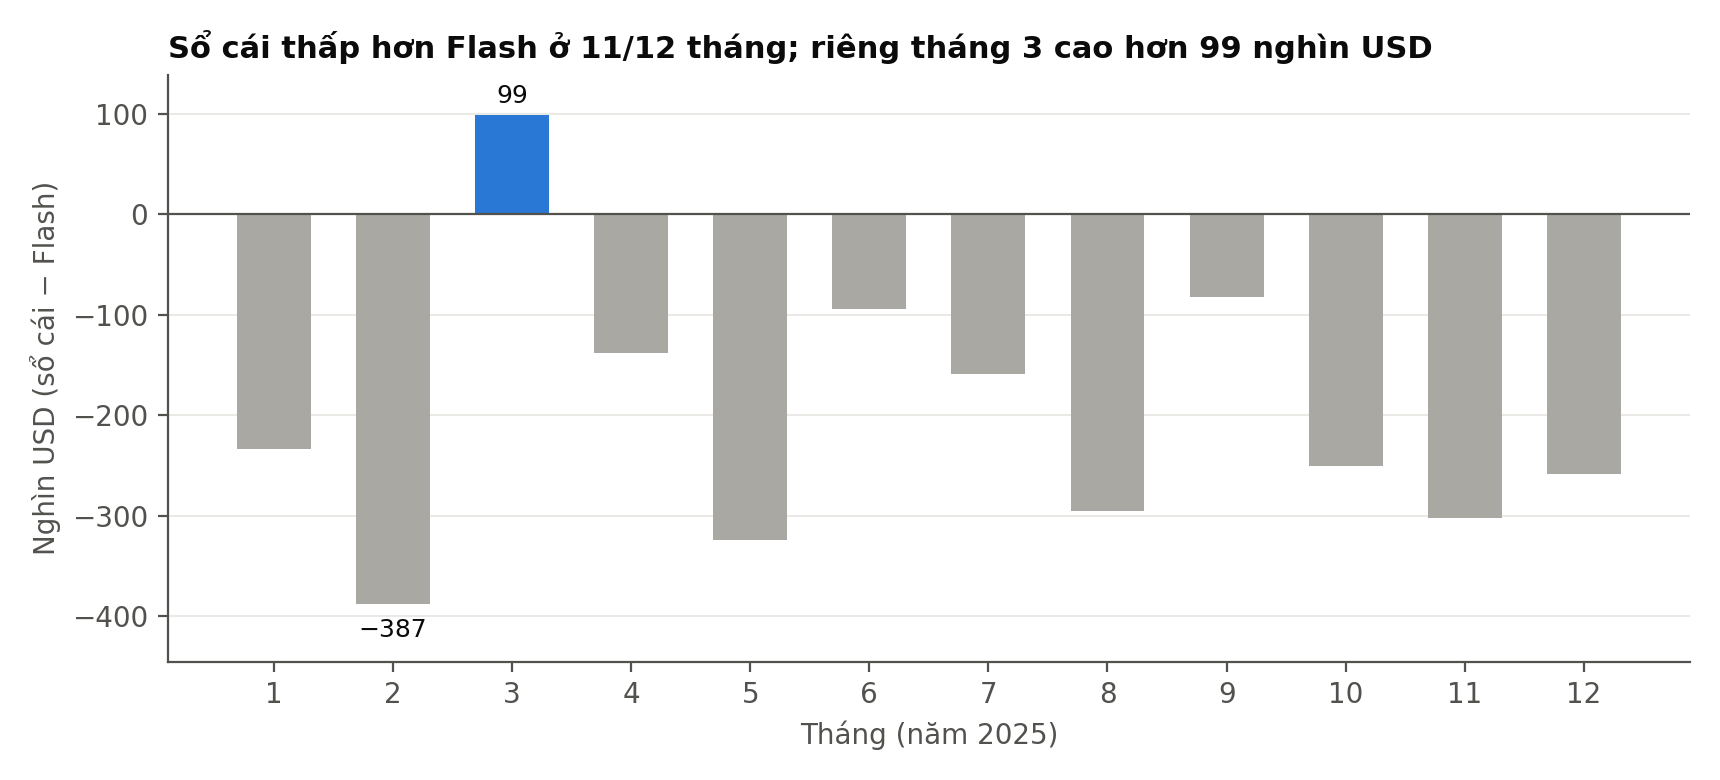
\includegraphics[width=0.95\textwidth]{generated/hinh_chenh_lech_thang.png}

\capfig{Chênh lệch sổ cái $-$ Flash theo tháng, nghìn USD \nguon{BR-Tổng}.}\label{fig:thang}
\end{figure}

Sổ cái thấp hơn Flash ở \SoThangThap{}/12 tháng (Hình~\ref{fig:thang}, Bảng~\ref{tab:thang}). Ba điểm cần giải thích ở phần sau:
\begin{itemize}
  \item \textbf{Tháng 3 đi ngược chiều}: sổ cái cao hơn Flash \SoThangBaChenhLech{} USD (+\SoThangBaPct). Nếu chênh lệch chỉ do chiết khấu và đơn hủy thì không tháng nào có thể dương, nên phải có một khoản theo thời điểm đẩy doanh thu vào tháng 3.
  \item \textbf{Mức lệch dao động mạnh} giữa các tháng: nặng nhất theo \% là \SoThangLechNhatPct{}, nặng nhất theo số tiền là \SoThangLechNhatTien{} USD.
  \item Chênh lệch cả năm là \SoChenhLechNam{} USD (\SoPctNam{} so với Flash).
\end{itemize}

\begin{table}[H]
\captab{Flash, sổ cái và chênh lệch theo tháng, USD \nguon{BR-Tổng}}\label{tab:thang}
\centering
\begin{tabular}{@{}l r r r r@{}}
\toprule
Tháng & Flash & Sổ cái & Chênh lệch & \% so với Flash \\
\midrule
Tháng 1 & 2.859.589 & 2.626.167,29 & $-$233.421,71 & $-$8,16\% \\
Tháng 2 & 3.490.159 & 3.102.906,99 & $-$387.252,01 & $-$11,10\% \\
Tháng 3 & 2.001.911 & 2.100.928,53 & 99.017,53 & 4,95\% \\
Tháng 4 & 1.035.907 & 898.049,36 & $-$137.857,64 & $-$13,31\% \\
Tháng 5 & 2.802.769 & 2.478.745,50 & $-$324.023,50 & $-$11,56\% \\
Tháng 6 & 2.506.912 & 2.412.461,84 & $-$94.450,16 & $-$3,77\% \\
Tháng 7 & 2.248.805 & 2.089.895,01 & $-$158.909,99 & $-$7,07\% \\
Tháng 8 & 2.569.740 & 2.274.164,62 & $-$295.575,38 & $-$11,50\% \\
Tháng 9 & 2.576.818 & 2.494.221,48 & $-$82.596,52 & $-$3,21\% \\
Tháng 10 & 2.743.824 & 2.493.635,92 & $-$250.188,08 & $-$9,12\% \\
Tháng 11 & 2.806.714 & 2.504.559,28 & $-$302.154,72 & $-$10,77\% \\
Tháng 12 & 3.481.253 & 3.222.760,41 & $-$258.492,59 & $-$7,43\% \\
\midrule
\textbf{Cả năm} & \textbf{31.124.401} & \textbf{28.698.496,23} & \textbf{$-$2.425.904,77} & \textbf{$-$7,79\%} \\
\bottomrule
\end{tabular}

\end{table}

\subsection{Theo kênh}

\begin{table}[H]
\captab{Flash, sổ cái và chênh lệch theo kênh cả năm, USD \nguon{BR-CH}, \nguon{BR-WEB}}\label{tab:kenh}
\centering
\begin{tabular}{@{}l r r r r@{}}
\toprule
Kênh & Flash & Sổ cái & Chênh lệch & \% so với Flash \\
\midrule
Cửa hàng & 14.060.500 & 13.181.898,25 & $-$878.601,75 & $-$6,25\% \\
Online & 17.063.901 & 15.515.347,98 & $-$1.548.553,02 & $-$9,08\% \\
Chưa gắn kênh & 0 & 1.250,00 & 1.250,00 & -- \\
\midrule
\textbf{Tổng} & \textbf{31.124.401} & \textbf{28.698.496,23} & \textbf{$-$2.425.904,77} & \textbf{$-$7,79\%} \\
\multicolumn{3}{@{}l}{\textit{Kiểm tra: sổ cái cửa hàng + online $-$ tổng sổ cái}} & \textit{$-$1.250,00} & \\
\bottomrule
\end{tabular}

\end{table}

Kênh online chiếm \SoOnlineTyTrong{} phần chênh lệch (\SoOnlineChenhLech{} USD), nhiều hơn kênh cửa hàng, dù doanh số online chỉ hơn cửa hàng khoảng một phần năm. Dòng kiểm tra ở cuối Bảng~\ref{tab:kenh} cho thấy sổ cái của hai kênh cửa hàng và online cộng lại \textbf{thiếu \SoChuaGanKenh{} USD} so với tổng sổ cái: đó là bút toán ADJ-0925 không gắn kênh nào. Khoản này chỉ lộ ra khi kiểm tra các phần có cộng đủ tổng hay không.

\subsection{Điều chưa biết sau bước khám phá}

Bảng tổng chỉ trả lời "lệch bao nhiêu". Nó chưa trả lời lệch do đâu, phần nào hợp lệ, phần nào là lỗi, và vì sao tháng 3 đi ngược chiều. Mục~IV tách chênh lệch thành từng khoản, bắt đầu từ mức chi tiết nhất: cửa hàng $\times$ ngày và đơn online $\times$ ngày giao.

\section{Phân tích chính: chênh lệch gồm những khoản nào}

\subsection{Đối soát cửa hàng theo ngày ghi sổ}
\choviet{store-recon}

\subsection{Đối soát online và hàng trả}
\choviet{web-return-recon}

\subsection{Năm lý do lệch, chứng minh bằng số}
\choviet{web-return-recon}

\subsection{Bảng cầu nối 12 tháng}
\choviet{bridge-monthly, bridge-template-log}

\subsection{Kiểm chứng bằng cách tính thứ hai}
\choviet{dax-bridge}

\subsection{Dashboard}
\choviet{dashboard}

\section{Phát hiện chính}
\choviet{conclusions}

\section{Đề xuất cải tiến quy trình}
\choviet{conclusions}

\section{Giới hạn và bước tiếp theo}
\choviet{conclusions}

\section{Tài liệu tham khảo}
\printbibliography[heading=none]


\clearpage
\section*{Phụ lục}
\addcontentsline{toc}{section}{Phụ lục}
\renewcommand{\thesubsection}{\Alph{subsection}.}
\setcounter{subsection}{0}

\subsection{Mã Power Query}
\choviet{report-draft}

\subsection{Nhật ký ngoại lệ đầy đủ}
Sinh từ truy vấn \texttt{q\_ExceptionLog} (sheet \texttt{Nhat\_ky\_du\_lieu}); sheet \texttt{Nhat\_ky\_ngoai\_le} của file mẫu đọc lại đúng bảng này. Cột ``Phát hiện ở bước'' và ``Nguồn'' xem trong file Excel.

{\scriptsize
\begin{longtable}{@{}L{0.85cm} L{4.05cm} r L{1.6cm} L{1.6cm} L{2.85cm} L{1.7cm}@{}}
\toprule
Mã & Mô tả & USD & Kỳ & Phân loại & Hướng xử lý & Phụ trách; trạng thái \\
\midrule
\endhead
EX-01 & Flash ghi giá niêm yết, sổ cái ghi giá sau giảm giá: tổng chiết khấu của mọi dòng POS và đơn online & $-$1.834.297,47 & 2025-01 đến 2025-12 & Quy tắc ghi nhận & Trình bày trong cầu nối; đề nghị Flash báo thêm doanh số sau giảm giá & Kinh doanh; Đã giải thích \\
EX-02 & 12 dòng POS trùng khóa ở cửa hàng NX007 (mã POS 74) ngày 29/03/2025: file POS xuất 2 lần, Flash đếm cả bản trùng & $-$12.622,20 & 2025-03 & Lỗi dữ liệu & Bỏ bản xuất sau; chặn xuất lặp ở hệ thống POS & IT; Cần sửa nguồn \\
EX-03 & 124 đơn online đặt trong kỳ rồi bị hủy: Flash có tính, sổ cái không ghi & $-$215.658,92 & 2025-01 đến 2025-12 & Quy tắc ghi nhận & Đề nghị Flash loại đơn hủy hoặc báo riêng & Kinh doanh; Đã giải thích \\
EX-04 & Đơn đặt và giao khác tháng trong năm: tháng này chuyển đi, tháng sau nhận lại; lớn nhất 2025-03 (281.787,98) & 0,00 & 2025-01 đến 2025-12 & Quy tắc ghi nhận & Không sửa; ghi chú trên Flash rằng doanh thu tính theo ngày đặt & Kinh doanh; Đã giải thích \\
EX-05 & 77 đơn đặt trước kỳ, giao trong kỳ: sổ cái có, Flash của kỳ không có & 122.107,89 & 2025-01 & Quy tắc ghi nhận & Không sửa; trình bày riêng khi so cả năm & Kinh doanh; Đã giải thích \\
EX-06 & 105 đơn đặt trong kỳ, giao sau kỳ: Flash có, sổ cái kỳ sau mới ghi & $-$174.705,79 & 2025-12 & Quy tắc ghi nhận & Theo dõi: sổ cái kỳ sau phải ghi nhận đủ số này & Tài chính; Đã giải thích \\
EX-07 & 65 dòng POS bán cuối tháng 2025-05 vào ngày nghỉ, ghi sổ tháng 2025-06: 41.464,78 USD chuyển tháng, tự bù trừ & 0,00 & 2025-05, 2025-06 & Quy tắc ghi nhận & Không sửa; tự bù trừ ở tháng sau & Tài chính; Đã giải thích \\
EX-08 & 101 dòng POS bán cuối tháng 2025-08 vào ngày nghỉ, ghi sổ tháng 2025-09: 75.240,30 USD chuyển tháng, tự bù trừ & 0,00 & 2025-08, 2025-09 & Quy tắc ghi nhận & Không sửa; tự bù trừ ở tháng sau & Tài chính; Đã giải thích \\
EX-09 & 101 dòng POS bán cuối tháng 2025-11 vào ngày nghỉ, ghi sổ tháng 2025-12: 80.588,85 USD chuyển tháng, tự bù trừ & 0,00 & 2025-11, 2025-12 & Quy tắc ghi nhận & Không sửa; tự bù trừ ở tháng sau & Tài chính; Đã giải thích \\
EX-10 & NX057 ngày 21/11/2025: POS có 7.227,56 USD nhưng sổ cái không có bút toán & $-$7.227,56 & 2025-11 & Lỗi dữ liệu & So ô cửa hàng × ngày trước khi khóa sổ; IT kiểm tra giao diện chuyển dữ liệu POS sang sổ cái & Tài chính, IT; Đã sửa kỳ sau \\
EX-11 & NX057 ngày 02/12/2025: sổ cái có bút toán JE20251206231 (POS\_CATCHUP) nhưng POS không có dòng nào & 7.227,56 & 2025-12 & Lỗi dữ liệu & So ô cửa hàng × ngày trước khi khóa sổ; IT kiểm tra giao diện chuyển dữ liệu POS sang sổ cái & Tài chính, IT; Đã sửa kỳ sau \\
EX-12 & 169 đơn bị trả, sổ cái ghi giảm vào ngày nhận hàng trả; Flash không trừ (tỷ giá ngày đặt) & $-$349.148,23 & 2025-01 đến 2025-12 & Quy tắc ghi nhận & Đề nghị tách báo cáo hàng trả bên cạnh Flash & Kinh doanh; Đã giải thích \\
EX-13 & 12 bút toán tay MJ-SHIP ghi phí vận chuyển vào doanh thu online; Flash không có khoản này & 94.766,95 & 2025-01 đến 2025-12 & Quy tắc ghi nhận & Trình bày riêng trong cầu nối & Tài chính; Đã giải thích \\
EX-14 & Bút toán tay MJ-RCL-2506 chuyển 3.480,00 USD doanh thu của NX019 sang kênh online; toàn công ty không đổi & 0,00 & 2025-06 & Quy tắc ghi nhận & Trình bày ở bảng cầu nối theo kênh & Tài chính; Đã giải thích \\
EX-15 & Flash đổi theo tỷ giá ngày đặt / ngày bán, sổ cái theo tỷ giá cuối tháng ghi sổ & $-$57.598,01 & 2025-01 đến 2025-12 & Quy tắc ghi nhận & Trình bày riêng một dòng; không sửa & Tài chính; Đã giải thích \\
EX-16 & Flash làm tròn từng dòng đến USD, sổ cái làm tròn từng bút toán đến 2 chữ số & 1,01 & 2025-01 đến 2025-12 & Sai số chấp nhận & Ghi một dòng, không đào thêm & Tài chính; Đã giải thích \\
EX-17 & Bút toán JE20250904892 (MJ-ADJ-2509) ghi 1.250,00 USD doanh thu, không gắn kênh, không có giấy tờ làm căn cứ & 1.250,00 & 2025-09 & Chưa giải thích được & Yêu cầu phòng Tài chính gửi chứng từ; không gán vào khoản khác & Tài chính; Chờ phản hồi \\
\midrule
& \textbf{Tổng (= chênh lệch sổ cái $-$ Flash cả năm)} & \textbf{$-$2.425.904,77} & & & & \\
\bottomrule
\end{longtable}}


\subsection{Bảng tra nhãn nguồn số liệu}

Mỗi kết luận trong báo cáo ghi kèm nhãn cho biết con số lấy từ bảng nào. Chữ viết tắt trong nhãn: QC (Quality Control, kiểm soát chất lượng), RC (Reconciliation, đối soát), BR (Bridge, cầu nối), EX (Exception, ngoại lệ), CH (cửa hàng), RET (Return, hàng trả).

\captab{Nhãn nguồn số liệu}\nopagebreak[4]
\begin{longtable}{@{}L{3.0cm} L{6.0cm} L{6.0cm}@{}}
\toprule
Nhãn & Bảng & Nơi xem trong file Excel Power Query \\
\midrule
\endhead
\nguon{QC} & Kiểm tra tổng, 5 bẫy, chất lượng dữ liệu & Sheet \texttt{Kiem\_tra}, \texttt{Bay\_du\_lieu}, \texttt{Chat\_luong\_du\_lieu}; truy vấn \texttt{q\_Check}, \texttt{q\_Traps}, \texttt{q\_DataQuality} \\
\nguon{RC-CH} & Đối soát cửa hàng: theo ngày ghi sổ (sheet \texttt{Doi\_soat\_CH\_ngay}), so với ngày bán (\texttt{So\_ngay\_ban\_ngay\_ghi\_so}), theo tháng có cờ vượt ngưỡng (\texttt{Doi\_soat\_CH\_thang}), lệch ngày ghi sổ (\texttt{Lech\_ngay\_ghi\_so}) & Truy vấn \texttt{q\_RC\_Store}, \texttt{q\_RC\_Store\_DayCompare}, \texttt{q\_RC\_Store\_Month}, \texttt{q\_RC\_Store\_Timing} \\
\nguon{RC-WEB} & Đối soát online: theo ngày giao $\times$ loại tiền (sheet \texttt{Doi\_soat\_online}), theo tháng có cờ vượt ngưỡng (\texttt{Doi\_soat\_online\_thang}), lệch thời điểm online (\texttt{Lech\_thoi\_diem\_online}); bảng 5 lý do (\texttt{Nam\_ly\_do}) và danh mục khoản, nhóm (\texttt{Danh\_muc\_khoan}) & Truy vấn \texttt{q\_RC\_Web}, \texttt{q\_RC\_Web\_Month}, \texttt{q\_Web\_Timing}, \texttt{q\_FiveReasons}, \texttt{q\_BridgeItems} \\
\nguon{RC-RET} & Đối soát hàng trả $\times$ ngày trả $\times$ loại tiền (sheet \texttt{Doi\_soat\_hang\_tra}) & Truy vấn \texttt{q\_RC\_Return} \\
\nguon{BR-Tổng} & Bảng cầu nối toàn công ty (dòng Flash, sổ cái: sheet \texttt{Chenh\_lech\_thang}) & Truy vấn \texttt{q\_BR\_Long}, cột \texttt{bridge} = COMPANY \\
\nguon{BR-CH},\newline \nguon{BR-WEB} & Bảng cầu nối cửa hàng, online (dòng Flash, sổ cái: sheet \texttt{Chenh\_lech\_kenh}) & Truy vấn \texttt{q\_BR\_Long}, cột \texttt{bridge} = STORE, WEB \\
\nguon{EX-xx} & Dòng xx của nhật ký ngoại lệ & Truy vấn \texttt{q\_ExceptionLog} \\
\bottomrule
\end{longtable}

\subsection{Ba phiên bản số làm tròn}

Đề có ba nguồn cho cùng một bảng cầu nối cả năm, khác nhau vài USD ở ba khoản (Bảng~\ref{tab:lamtron}). Tổng các khoản luôn đúng bằng chênh lệch; khác nhau chỉ ở chỗ phần làm tròn nằm ở dòng nào.

\begin{table}[H]
\captab{Ba phiên bản của ba khoản cầu nối cả năm, USD}\label{tab:lamtron}
\centering
\begin{tabular}{@{}L{7.2cm} r r r@{}}
\toprule
Nguồn & Chiết khấu & Tỷ giá & Làm tròn \\
\midrule
Nhóm: đổi tiền từ nội tệ $\div$ tỷ giá, không làm tròn từng dòng (định nghĩa slide 34) & \SoBRChietKhau{} & \SoBRTyGia{} & +\SoBRLamTron{} \\
Slide 32 & $-$1.834.297 & $-$57.598 & +1,01 \\
Dashboard mẫu của mentor: cộng các cột USD đã làm tròn sẵn từng dòng & $-$1.834.298,38 & $-$57.598,50 & +2,33 \\
\bottomrule
\end{tabular}
\end{table}

Lý do nhóm chọn cách đầu: dòng làm tròn khi đó chỉ gồm phần Flash làm tròn từng dòng đến USD (khoảng +0,95) và phần sổ cái làm tròn từng bút toán đến 2 chữ số (khoảng +0,05), đúng nghĩa ``làm tròn'', và mỗi tháng không quá \SoBRLamTronMax{} USD (ngưỡng 5 USD). Số của nhóm ở bảng này lấy từ bảng cầu nối Power Query \nguon{BR-Tổng}; bảng tính kiểm tra viết bằng Python ra cùng số.

\subsection{So sánh khi đổi thứ tự các bước cầu nối}
Cùng một khoản lệch có thể ra số khác nhau tùy bước nào tính trước, dù tổng các khoản không đổi (Bảng~\ref{tab:doithutu}). Ví dụ dòng POS trùng tính trước chiết khấu thì thành \SoDoiTrungMoi{} USD (theo giá trước giảm giá); hàng trả tính sau tỷ giá thì thành \SoDoiTraMoi{} USD (theo tỷ giá ngày trả), còn dòng tỷ giá thành \SoDoiTyGiaMoi{}. Vì vậy thứ tự các bước được chốt trước khi tính và ghi rõ trong quy ước. Nhóm chọn tính chiết khấu trước mọi khoản khác để các khoản sau đều đo theo giá thực bán, và đổi mọi khoản theo tỷ giá ngày đặt để toàn bộ phần do tỷ giá nằm ở một dòng.

\begin{table}[H]
\captab{Số của hai khoản khi đổi thứ tự các bước, USD cả năm toàn công ty \nguon{BR-Tổng}}\label{tab:doithutu}
\centering
{\small
\begin{tabular}{@{}l r r r@{}}
\toprule
Cách đổi thứ tự và khoản bị ảnh hưởng & Thứ tự đã chốt & Khi đổi & Thay đổi \\
\midrule
\multicolumn{4}{@{}l}{\textit{1. Tính dòng POS trùng trước chiết khấu (theo giá trước giảm giá)}} \\
\quad Dòng POS bị trùng & $-$12.622,20 & $-$13.695,13 & $-$1.072,93 \\
\quad Chiết khấu & $-$1.834.297,47 & $-$1.833.224,54 & 1.072,93 \\
\midrule
\multicolumn{4}{@{}l}{\textit{2. Tính đơn hủy trước chiết khấu (theo giá trước giảm giá)}} \\
\quad Đơn online bị hủy & $-$215.658,92 & $-$230.286,39 & $-$14.627,47 \\
\quad Chiết khấu & $-$1.834.297,47 & $-$1.819.670,00 & 14.627,47 \\
\midrule
\multicolumn{4}{@{}l}{\textit{3. Tính tỷ giá trước hàng trả (hàng trả theo tỷ giá ngày trả)}} \\
\quad Hàng trả lại & $-$349.148,23 & $-$349.652,76 & $-$504,53 \\
\quad Tỷ giá & $-$57.598,01 & $-$57.093,48 & 504,53 \\
\bottomrule
\end{tabular}}

\end{table}

\subsection{Khai báo dùng AI}

Nhóm dùng trợ lý AI (trí tuệ nhân tạo) Claude để viết nháp code Power Query, DAX, script kiểm tra và một phần lời văn. Mỗi phần việc có một file plan trong thư mục \texttt{plans/} ghi rõ: nhờ AI làm gì, phần nào do AI viết ra, và nhóm kiểm tra lại bằng cách nào (so với bảng tổng kiểm soát của đề, với slide, với một cách tính độc lập). Bảng tổng hợp đầy đủ:
\choviet{report-draft}


\end{document}
